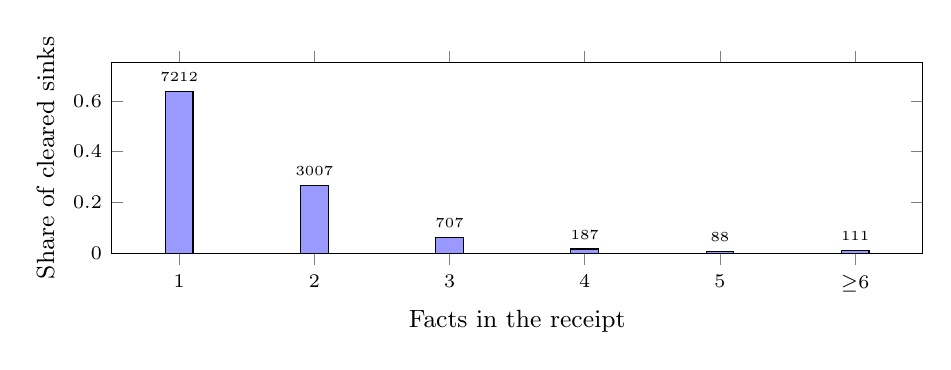
\begin{tikzpicture}
\begin{axis}[ybar, width=0.98\linewidth, height=4cm, bar width=10pt, ymin=0, ymax=0.75,
  symbolic x coords={1,2,3,4,5,6}, xticklabels={1,2,3,4,5,$\geq$6}, xtick=data,
  xlabel={Facts in the receipt}, ylabel={Share of cleared sinks}, nodes near coords, nodes near coords style={font=\tiny},
  point meta=explicit symbolic, tick label style={font=\scriptsize}, label style={font=\small}]
\addplot[fill=blue!40] coordinates {(1,0.6376) [7212] (2,0.2658) [3007] (3,0.0625) [707] (4,0.0165) [187] (5,0.0078) [88] (6,0.0098) [111]};
\end{axis}
\end{tikzpicture}
